\section{Quantum Optics} \label{chap:quantum-optics}
This chapter introduces concepts in \textit{Quantum Optics}. The implementation of quantum computers we discuss in this manuscript has a qubit which is a two level system\footnote{Often I'll use the words "atom" and "qubit" interchangeably. The qubit acts as a two level atom} interacting with light (both classical and quantum) inside a resonating cavity.

\subsection{Dirac's Method for Canonical Quantization}
Before we dive into anything new, we'll start by going over the method to quantize any oscillating phenomena introduced by Paul Dirac in his 1925 Ph.D. dissertation.

Any system of which we have a classical description can be quantized following a process known as canonical quantization. A classical system can be described by pairs of \textit{canonically conjugate variables}, $ (q_j, p_j)$ satisfying the Hamilton equations
\begin{align*}
    &\dot{q_j} =\quad \frac{\partial H}{\partial p_j} \\
    &\dot{p_j} = -\frac{\partial H}{\partial q_j}
\end{align*}
$q_j$ is called    the \textit{canonical coordinate} and $p_j$ is called the \textit{canonically conjugate momentum to the coordinate $q_j$}.

To quantize the system we need to replace the dynamical variables $ (q_j, p_j)$ with canonically conjugate operators $ (\hat{q_j}, \hat{p_j})$ satisfying the commutation relation 
\[
[\hat{q}_j, \hat{q}_k] = [\hat{p}_j, \hat{p}_k] = 0 \quad  \text{and} \quad [\hat{q}_j, \hat{p}_k] = i\hbar \delta_{jk}
\]
The Hamiltonian of the quantum system is obtained by replacing the classical Hamiltonian $E = H (q_1,p_1, \dots ,q_j, p_j, \dots)$ with the quantum Hamiltonian $\hat{H} = H (\hat{q_1},\hat{p_1}, \dots ,\hat{q_j}, \hat{p_j}, \dots)$. 
%We know that we can get any physical observable and the time evolution of states from the Hamiltonian using the schr\"{o}dinger equation. If we have the Hamiltonian, we have everything.

Dirac's method is best used to solve the system of the quantum harmonic oscillator. The Hamiltonian of the system is
\[
    \hat{H} = \frac{\hat{p}^2}{2m} + \frac{1}{2}m\omega^2 \hat{q}^2
\]
To solve it you introduce the annihilation and creation operators (Also called the "ladder operators"), $\hat{a}$ and $\hat{a}^\dag$ respectively. The ladder operators satisfy the commutation relation $[\hat{a}, \hat{a}^\dag] = 1$. Since $\hat{a} \ne \hat{a}^\dag$, these operators are not hermitian and therefore not observables of the system, but every observable of the system can be expressed using them. The operators are
\begin{align*}
    \hat{a} = \sqrt{\frac{m \omega}{2\hbar}} (\hat{q} + \frac{i}{m\omega}\hat{p}) \\
    \hat{a}^\dag = \sqrt{\frac{m \omega}{2\hbar}} (\hat{q} - \frac{i}{m\omega}\hat{p})
\end{align*}
The Hamiltonian is therefore
\[
    \hat{H} = \hbar \omega (\hat{a}^\dag\hat{a} + \frac{1}{2})
\]
The energy eigenstates are denoted $\ket{0}, \ket{1}, \ket{2}, \dots$ where $\ket{n}$ is the eigen state of the $n^{th}$ energy level, $E_n$. A set of  important relations between the eigenstates the the ladder operators are
\begin{align*}
    &\hat{a}^\dag \ket{n} = \sqrt{n+1}\ket{n+1} \\
    &\hat{a} \ket{n} = \sqrt{n}\ket{n-1} \\
    &\hat{a} \ket{0} = 0
\end{align*}
From these relations the ladder operators get their name, since you can think of them as ways to climb up and down the energy "ladder". These eigenstates are called the \textbf{number states} or \textbf{Fock states} after Vladimir Fock who developed this representation. The number states $\ket{n}$ are also the eigenstates of the \textit{number operator} $\hat{N} = \hat{a}^\dag\hat{a}$, with eigenvalue $n$, $\hat{N}\ket{n} =  n\ket{n}$, hence the name.

\subsection{The Quantization of the Electromagnetic Field}
\subsubsection{The Homogeneous Electromagnetic Equation}
Maxwell's equations in free space are
\begin{subequations}
    \label{eq:optim}
    \begin{align}
        &\grad \cdot \textbf{E} = 0 \label{eq:Maxwell-1} \\
        &\grad \cdot \textbf{B} = 0 \label{eq:Maxwell-2}\\
        &\grad \cross \textbf{E} = \frac{\partial\textbf{B}}{\partial t} \label{eq:Maxwell-3}\\
        &\grad \cross \textbf{B} = \mu_0 \epsilon_0 \frac{\partial\textbf{E}}{\partial t} \label{eq:Maxwell-4}
    \end{align}
\end{subequations}
Taking the curl of \ref{eq:Maxwell-3} and \ref{eq:Maxwell-4} yields
\begin{subequations} 
\label{eq:curl-}
    \begin{align}
        &\curl{ (\curl{\textbf{E}})} 
        = \curl{ (-\frac{\partial \textbf{B}}{\partial t})} 
        = -\frac{\partial}{\partial t} (\curl{\textbf{B}})
        = - \mu_0 \epsilon_0 \frac{\partial^2 E}{\partial t^2} 
        \label{eq:curl-E}\\
        &\curl{ (\curl{\textbf{B}})} 
        = \curl{ (\mu_0 \epsilon_0 \frac{\partial E}{\partial t})} 
        = \mu_0 \epsilon_0\frac{\partial}{\partial t} (\curl{E}) 
        = - \mu_0 \epsilon_0 \frac{\partial^2 \textbf{B}}{\partial t^2} 
        \label{eq:curl-B}
    \end{align}
\end{subequations}
   
Using the vector identity
\begin{equation}
    \nabla \times \left ( \nabla \times \mathbf{V} \right) = \nabla \left ( \nabla \cdot \mathbf{V} \right) - \nabla^2 \mathbf{V}
\end{equation}
We obtain from \ref{eq:curl-E} and \ref{eq:curl-B}
\begin{subequations}
    \begin{align}
        &\nabla (\nabla \cdot \textbf{E}) - \nabla^2 \textbf{E} 
        = -\mu_0\epsilon_0\frac{\partial^2 \textbf{E}}{\partial t^2} \\
        &\nabla (\nabla \cdot \textbf{B}) - \nabla^2 \textbf{B} 
        = -\mu_0\epsilon_0\frac{\partial^2 \textbf{B}}{\partial t^2}
    \end{align}
\end{subequations}
Using \ref{eq:Maxwell-1} and \ref{eq:Maxwell-2} to cancel the left most term we get
\begin{subequations}
    \begin{align}
        &\nabla^2 \textbf{E} = \mu_0\epsilon_0\frac{\partial^2 \textbf{E}}{\partial t^2}\\
        &\nabla^2 \textbf{B} = \mu_0\epsilon_0\frac{\partial^2 \textbf{B}}{\partial t^2}
    \end{align}
\end{subequations}
Replacing $v_{ph} = \frac{1}{\sqrt{\mu_0\epsilon_0}}$ with $c$ since the phase velocity is the speed of light for electromagnetic radiation in vacuum
\begin{equation} \label{eq:Homo_electro_wave}
    \begin{split}
        \nabla^2 \textbf{E} = \frac{1}{c^2}\frac{\partial^2 \textbf{E}}{\partial t^2} \\
        \nabla^2 \textbf{B} = \frac{1}{c^2}\frac{\partial^2 \textbf{B}}{\partial t^2}
    \end{split}
\end{equation}

These equation are called \textit{the homogeneous electromagnetic wave equations}.
We'll pick a polarization, arbitrarily, to be in the x direction. The equations become
\begin{equation} \label{eq:Homo_electro_wave_pol}
    \begin{split}
        \frac{\partial^2 E_x}{\partial x^2} = \frac{1}{c_0^2}\frac{\partial^2 E_x}{\partial t^2} \\
        \frac{\partial^2 B_y}{\partial y^2} = \frac{1}{c_0^2}\frac{\partial^2 B_y}{\partial t^2} 
    \end{split}
\end{equation}

\subsubsection{The Single Mode Cavity}
Now that we have the homogeneous electromagnetic field equations at hand we can solve them.
We solve \ref{eq:Homo_electro_wave_pol} using separation of variables,
\[
    E_x (z, t)= Z (z)T (t)
\]
Yielding the solution,\footnote{We've skipped several of steps going from the differential equation to their solutions, mainly it is not clear how the scalar constant in front of the expression got there, it has to do with the fact that the total energy of the electromagnetic field is given by $H = \frac{\epsilon_0}{2} \int_V \textbf{E}^2 + c^2 \textbf{B}^2 d^3 r$. We won't go into the calculations because they make it much more complicated and doesn't give much more insights into the physics}
\begin{equation}
    \begin{split}
        E_x (z, t) = \sqrt{\frac{2 \omega_c^2}{V \epsilon_0}}q (t)\sin{kz} \\
        B_y (z, t) = \sqrt{\frac{2 \mu_0}{V}}\dot{q} (t)\cos{kz}
    \end{split}
\end{equation}
where $V$ is the effective volume of the cavity, $q$ is a time-dependent amplitude with units of length, $k = m\pi/L$ for
an integer $m > 0$, and $\omega_c$ is the frequency of the mode.

The Hamiltonian of a single mode is hence given by
\begin{align}
    H &= \frac{1}{2}\int\epsilon_0 \textbf{E}^2 + \frac{\textbf{B}^2}{\mu_0} dV \\
    &= \frac{1}{2}\int\epsilon_0 E_x^2 (z, t) + \frac{B_y^2 (z, t)}{\mu_0} dz \\
    &= \frac{1}{2}[\dot{q}^2 (t) + \omega_c^2 q^2 (t)]
\end{align}
Going from dynamical variables to operators, $\hat{q}$ and $\hat{p}$ that satisfy the commutation relation $[\hat{q}, \hat{p}] = i\hbar$, we get
\begin{align}
     &\hat{E}_x (z, t) = \sqrt{\frac{2 \omega_c^2}{V \epsilon_0}}\hat{q} (t)\sin{kz} \\
     &\hat{B}_y (z, t) = \sqrt{\frac{2 \mu_0}{V}}\hat{p} (t)\cos{kz} \\
     &\hat{H} = \frac{1}{2}[\hat{p}^2 (t) + \omega_c^2 \hat{q}^2 (t)]
\end{align}
This is the same Hamiltonian as for the harmonic oscillator. \textbf{Electromagnetic radiation acts as a harmonic oscillator}.

Let’s introduce creation and annihilation operators
\begin{align*}
    \hat{a} (t) = \frac{1}{\sqrt{2\hbar\omega_c}}[\omega_c\hat{q} (t) + i\hat{p} (t)] \\
    \hat{a}^\dag (t) = \frac{1}{\sqrt{2\hbar\omega_c}}[\omega_c\hat{q} (t) - i\hat{p} (t)]
\end{align*}

In term of the creation and annihilation operators, the electric and magnetic field operators become
\begin{align}
         &\hat{E}_x (   z, t) = E_0[\hat{a} (t) + \hat{a}^\dag (t)]\sin{kz} \\
         &\hat{B}_y (z, t) = \frac{E_0}{c}[\hat{a} (t) - \hat{a}^\dag (t)]\cos{kz}
\end{align}
And we can write the Hamiltonian as
\begin{equation}\label{eq:cavity_hamiltonian}
    \hat{H}_{cavity} = \hbar\omega_c[\hat{a}\hat{a}^\dag + \frac{1}{2}] \approx \hbar\omega_c\hat{a}\hat{a}^\dag
\end{equation}
Ignoring the zero-point energy $\frac{\hbar\omega_c}{2}$.

Since the eigenstates of the quantum harmonic oscillator are the number states $\ket{n}$, they are also the eigenstates of electromagnetic radiation. We can show that the momentum operator of electromagnetic radiation takes the form $\hat{P} = \hbar \textbf{k} \hat{a}^\dag \hat{a}$. Where $\textbf{k}$ is the wave number of the electromagnetic wave. Applying the momentum operator to the number states we  see that
\[
    \hat{P}\ket{n} =  \hbar \textbf{k} \hat{a}^\dag \hat{a} \ket{n} = n\hbar \textbf{k}\ket{n}
\]
This is an important result, \textbf{the $\ket{n}$ state has well defined energy and momentum, same as $n$ particles, each with energy $\hbar \omega$ and momentum $\hbar \textbf{k}$, we call these particles \textit{photons}.} Hopefully you now see why these are called number states, they correspond to the \textit{number of photons in the cavity}.

\subsection{The Jaynes–Cummings Model}
Our goal is to mathematically model the Hamiltonian of a system of a two-level system, such as an atom, interacting with a single quantized mode of an electromagnetic field inside an optical cavity. First we'll divide the system into 3 parts, The atom, the cavity, and the interaction between them.
% http://aliramadhan.me/files/jaynes-cummings-model.pdf

\subsubsection{The Hamiltonians} \label{sec:the-hamiltonians}
We separate the Hamiltonian as
\[
    H = H_{atom} + H_{cavity} + H_{interaction}
\]
We'll now calculate each Hamiltonian separately

\paragraph*{cavity}
We already calculated the Hamiltonian of the cavity and it is given by equation \ref{eq:cavity_hamiltonian} as
\begin{equation}
    \boxed{\hat{H}_{cavity} = \hbar\omega_c\hat{a}\hat{a}^\dag}
\end{equation}


\paragraph*{atom}
The atom is a two-level system, meaning its state is in a general superposition of the ground, $\ket{g}$, and excited, $\ket{e}$, states. We know that $\hat{H}\ket{\psi} = E_\psi \ket{\psi}$ for every energy eigenstate, with energy $E_\psi$. We can use these eigenstates to spectrally decompose the Hamiltonian, $\hat{H} = \sum_\psi E_\psi \ket{\psi}\bra{\psi}$. In our case, with only ground and excited states, the Hamiltonian is
\begin{equation}
    \hat{H}_{atom} = E_g\ket{g}\bra{g} + E_e\ket{e}\bra{e}
\end{equation}
Using the vector representation of these states we'll write
\begin{align*} 
    \hat{H}_{atom} &= 
    E_e \begin{bmatrix}
    1 & 0     \\
    0   & 0   \\
    \end{bmatrix}
    + E_g \begin{bmatrix}
    0 & 0     \\
    0   & 1   \\
    \end{bmatrix} = 
    \begin{bmatrix}
    E_e & 0     \\
    0   & E_g   \\
    \end{bmatrix} \\
    % &= \frac{1}{2}\begin{bmatrix}
    % E_g + E_e & 0          \\
    % 0         & E_g + E_e  \\
    % \end{bmatrix} +
    % \frac{1}{2}\begin{bmatrix}
    % E_e - E_g & 0          \\
    % 0         & - (E_e - E_g)  \\
    % \end{bmatrix} \\
    % &= \frac{1}{2} (E_g + E_e)\begin{bmatrix}
    % 1 & 0          \\
    % 0         & 1  \\
    % \end{bmatrix} +
    % \frac{1}{2} (E_e - E_g)\begin{bmatrix}
    % 1 & 0          \\
    % 0         & -1  \\
    % \end{bmatrix} \\
    &= \frac{1}{2} (E_g + E_e)\mathbb{I} + \frac{1}{2} (E_e - E_g)\hat{\sigma}_z
\end{align*}
Again, we define the zero point energy so that the first term becomes $0$. The energy difference is associated with a frequency $\omega_a$ and from the de-broglie relations $E = \hbar\omega$ so $E_e - E_g = \hbar\omega_a$. The atom Hamiltonian is therefore
\begin{equation}
    \boxed{\hat{H}_{atom} = \frac{1}{2}\hbar\omega_a\hat{\sigma}_z}
\end{equation}

\paragraph*{interaction}
The atom-cavity coupling comes from the interaction between the atomic dipole, $\hat{\textbf{d}}$, and the electric field of the cavity mode, $\hat{\textbf{E}}$. The corresponding Hamiltonian is
\[
\hat{H}_{interaction} = -\hat{\textbf{d}}\cdot\hat{\textbf{E}} = -\hat{d} E_0 \sin{kz} (\hat{a} + \hat{a}^\dag{})
\]
Where we assumed that the atomic dipole and electric field are parallel\footnote{Since the electric field creates the dipole in the direction of the field}.
We'll introduce the atomic transition operators
\[
    \hat{\sigma}_+ = \ket{e}\bra{g}, \quad\quad \hat{\sigma}_- = \ket{g}\bra{e} = \hat{\sigma}_+^{\dag{}}
\]

Due to parity selection rules, only the off-diagonal, only the off-diagonal elements of the dipole operator are nonzero so we may write
\[
    \hat{d} = d\ket{e}\bra{g} + d^* \ket{g}\bra{e} = d\hat{\sigma}_- + d^* \hat{\sigma}_+ = d (\hat{\sigma}_+ + \hat{\sigma}_-)
\]
Thus, the interaction Hamiltonian is
\begin{equation}
    \hat{H}_{interaction} = \hbar\Omega (\hat{\sigma}_+ + \hat{\sigma}_-) (\hat{a} +  \hat{a}^\dag) 
    = \hbar\Omega (\hat{\sigma}_+\hat{a} + \hat{\sigma}_+\hat{a}^\dag + \hat{\sigma}_-\hat{a} + \hat{\sigma}_-\hat{a}^\dag) 
\end{equation} \label{eq:interaction-hamiltonian}
Where $\Omega = -\frac{d}{\hbar}\sqrt{\frac{\hbar \omega_c}{\epsilon_0 V}} \sin (kz)$ is the amplitude of the interaction.
From \ref{eq:cavity_hamiltonian} the cavity ladder operators $\hat{a}$ and $\hat{a}^\dag$ evolve as
\begin{equation}
    \hat{a} (t) = \hat{a} (0)e^{-i\omega_c t}, \quad\quad \hat{a}^\dag{} (t) = \hat{a}^\dag{} (0)e^{i\omega_c t}
\end{equation}
And similarly we can show for the free evolution of the atom
\begin{equation}
    \hat{\sigma}_{\pm} (t) =   \hat{\sigma}_{\pm} (0)e^{\pm i\omega_a t}
\end{equation}
We can write while approximating $\omega_c \approx \omega_a$
\begin{equation}
    \begin{split}
        &\hat{\sigma}_+\hat{a} \sim e^{i (\omega_0 - \omega)t}\\
        &\hat{\sigma}_-\hat{a}^\dag \sim e^{-i (\omega_0 - \omega)t}\\
        &\hat{\sigma}_+\hat{a}^\dag \sim e^{i (\omega_0 + \omega)t}\\
        &\hat{\sigma}_-\hat{a} \sim e^{-i (\omega_0 + \omega)t}
    \end{split}
\end{equation}
We can see that the last two term vary much more rapidly than the first two. Furthermore, the last two terms do not conserve energy (They correspond to \textit{[photon addition + atom excitation]} and \textit{[photon reduction + atom relaxation]}). Therefore, we can drop the quickly rotating terms\footnote{This is called the \textit{Rotating Wave Approximation} or RWA in short}, yielding
\begin{equation} \label{eq:interaction-hamiltonian-RWA}
    \boxed{H_{interaction} = \hbar\Omega (\hat{\sigma}_+\hat{a} + \hat{\sigma}_-\hat{a}^\dag)}
\end{equation}

\par

Finally, we can write the full JC Hamiltonian
\begin{equation} \label{eq:JC-hamiltonian}
    \boxed{\hat{H} = \frac{1}{2}\hbar \omega_0\hat{\sigma}_z 
                     + \hbar \omega \hat{a}^\dag \hat{a} 
                     +  \hbar\Omega (\hat{\sigma}_+\hat{a} + \hat{\sigma}_-\hat{a}^\dag)}
\end{equation}


\subsubsection{Interaction with a Classical Field} \label{sec:interaction-with_classical-field}
As you might have noticed, we are classical creatures, I'm (fortunately) not in a superposition of being dead and alive at the same time. As classical creatures, if we want to interact with the quantum world we need to do so with classical means, with a classical interface to the quantum world. Back to the Jaynes-Cummings model, what happens when we introduce a classical electromagnetic field (such as the microwave drives that control the superconducting system)?

We can do the full rigorous way to calculate the interactions between the quantized atom and the classical electromagnetic field, but instead, we can use a "hack"\footnote{The "hack" is that, like we can turn a classical equation into a quantum one, by replacing dynamical variables with operators, we can do the same thing but in reverse. Taking a quantum expression and turning it into a classical one, by replacing operators with dynamical variables} to make the calculations much simpler, since we already calculated the interaction between the atom and the \textit{quantized} electromagnetic field. The Hamiltonian of the full quantum interaction, as given in equation \ref{eq:interaction-hamiltonian} is
\[
    H_{interaction} = \hbar \Omega (\hat{\sigma}_+ + \hat{\sigma}_-) (\hat{a} + \hat{a}^\dag)
\]
We can go from the quantized field to the classical field by simply replacing the field operators with dynamical variables representing the strength of the field, $\hat{a} \rightarrow a$ and $\hat{a}^\dag \rightarrow a^*$. We can also replace $\hat{\sigma}_+ + \hat{\sigma}_-$ with the Pauli matrix $\hat{\sigma}_x$ and get
\begin{equation}\label{eq:atom-field-class-int}
    H_{classical} = \hbar \Omega a \cdot \hat{\sigma}_x
\end{equation}

The transition from the middle term to the right term is allowed since we know that the Pauli matrices are observable quantities, hence are hermitian conjugates of themselves. $a$ is the amplitude of the classical field, later we'll replace it with $\epsilon_I (t)$ and $\epsilon_Q (t)$ for the drive fields since the classical field is not constant and it is, in fact, what we control in the system, but I'm getting ahead of myself, more on this will be shown in the optimal control chapter \ref{chap:optimal}.

\subsubsection{Effective Hamiltonian in the Dispersive Limit} \label{sec:dispersive}
As we've in appendix \ref{appen:annalytic}, when an atom interacts with a classical electromagnetic field, it oscillates between higher and lower energy states. These oscillations are the so called \textbf{\textit{Rabi Oscillations}} and are an important result in the atom-photon interaction theory. There is one catch though, if the electromagnetic field doesn't have \textbf{exactly} the same  energy as the energy difference between the two levels of the atom, the atom will never reach fully the higher energy state (see figure \ref{fig:rabi-oscillations}). The difference between the energy of the electromagnetic field, and  the atom  energy difference is called the detuning, $\Delta = \omega_{field} - \omega_{atom} = \frac{E_{field} - E_{atom}}{\hbar}$. The dispersive limit occurs when the detuning is very large compared  to the frequencies (in terms of the variables used in appendix \ref{appen:annalytic}, the limit is for $\Delta \gg \Omega_0$).

We are now going to consider the energies of the states $\ket{g, n}$ and $\ket{e, n+1}$, for any $n$. The energies are the eigenvalues of the Hamiltonian\footnote{Sometimes referred to as the \textit{time independent schr\"{o}dinger equation} $\hat{H}\ket{\psi} = E_n \ket{\psi}$, although this is an inaccurate name}. We can write this Hamiltonian as
\[
    \hat{H}_n = \frac{\hbar}{2} (\Delta \hat{\sigma}_z + \Omega_n \hat{\sigma}_y) + \hbar \omega_0 (n + \frac{1}{2})\hat{I}
\]

Where $\Omega_n = \Omega_0 \sqrt{n + 1}$.

The eigenvalues of this operator are
\[
    E_n^\pm = \hbar \omega_0 (n + \frac{1}{2}) \pm \frac{\hbar}{2}\sqrt{\Delta^2 +\Omega_n^2}
\]
Where the $\pm$ is $+$ for the ground state of the atom and $-$ for it's excited state. For $\Delta \gg \Omega_n$ we can approximate the square root as a Taylor series, and the overall expression is
\[
    E_n^\pm = \hbar \omega_0 (n + \frac{1}{2}) \pm (\frac{\Delta}{2} + \frac{\Omega_n^2}{\Delta}) =  \hbar \omega_0 (n + \frac{1}{2}) \pm (\frac{\Delta}{2} + \frac{ (n+1)\Omega_0^2}{\Delta})
\]
We can replace the number $n$ with the operator $\hat{n} = \hat{a}^\dag \hat{a}$. Moreover, the operator $\hat{\sigma}_z$ can be used to "replace" the $\pm$, since it's eigenvalue is $+1$ for the ground state and $-1$ for the excited state. The overall Hamiltonian is of the form
\begin{equation} \label{eq:dispersive-hamiltonian}
    \hat{H}_{\text{eff}} = \hbar \omega_0 \hat{a}^\dag \hat{a} + \frac{\Delta^2 + \Omega_0^2}{2\Delta}\hat{\sigma}_z + \frac{\Omega_0^2}{\Delta} \hat{a}^\dag \hat{a} \hat{\sigma}_z
\end{equation}
The physical interpretation of this new expression is that the frequency of the cavity changes by $\chi = 2\frac{\Omega^2}{\Delta}$ depending on the state of the atom. Or equivalently, the atom transition frequency changes by $\chi$ for each additional photon in the cavity.

% \subsection{Fock States (Number States)}
% % As always in quantum mechanics, when we have the Hamiltonian of the system we want to to it's eigenvalues, corresponding to the quantized energies of the system, and the eigenvectors, that form a complete basis of the space of states.

% We know that the Hamiltonian of a single mode in a cavity is given by
% \[
%     \hat{H} = \hbar \omega (\hat{a}^\dag \hat{a} + \frac{1}{2}) \quad \text{with} \quad [\hat{a}, \hat{a}^\dag] = 1
% \]
% The eigenequation is
% \[
%     \hat{H}\ket{\psi_n} = E_n \ket{\psi_n}
% \]
% We know that the eigenvalues of the equation are
% \[
%     E_n = \hbar \omega (n + \frac{1}{2}) \quad \text{with} \quad n = 0, 1, 2, \dots
% \]
% it is customary to write the eigenvectors as $\ket{n} := \ket{\psi_n}$. We know that they satisfy the equations
% \begin{align*}
%     &\hat{a}^\dag \ket{n} = \sqrt{n+1}\ket{n+1} \\
%     &\hat{a} \ket{n} = \sqrt{n}\ket{n-1} \\
%     &\hat{a}\ket{0} = 0
% \end{align*}
% The eigenvectors of the Hamiltonian are also the eigenvectors of the \textit{number operator}, $\hat{N} = \hat{a}^\dag \hat{a}$ in the eigenequation
% \[
%     \hat{N}\ket{n} = n\ket{n}
% \]
% these eigenvectors are called \textit{number states} or \textit{Fock states} after Vladimir Fock who developed this representation.

% We can show that the momentum operator of electromagnetic radiation takes the form $\hat{P} = \hbar \textbf{k} \hat{a}^\dag \hat{a}$. Where $\textbf{k}$ is the wave number of the electromagnetic wave. Applying the momentum operator to the number states we  see that
% \[
%     \hat{P}\ket{n} =  \hbar \textbf{k} \hat{a}^\dag \hat{a} \ket{n} = n\hbar \textbf{k}\ket{n}
% \]
% This is an important result, \textbf{the $\ket{n}$ state has well defined energy and momentum, same as $n$ particles, each with energy $\hbar \omega$ and momentum $\hbar \textbf{k}$, we call these particles \textit{photons}.} Hopefully you now see why these are called number states, they correspond to the \textit{number of photons in the cavity}.

\subsection{Visualizing Quantum States}
As you'll soon find out in the optimal control chapter, we're going to develop a system that is some sort of a \textit{black box}. We can't really control directly how it works, we can only make indirect changes to try to get everything to work\footnote{This is the nature of numerical optimization problems}.

This is why we want to get as much insight about the system as we can, and understand that insight in a way that allows us to create intelligent changes to the system according to the data we gather. Visualization of quantum states give us a better understanding of the system performance, and allows us to better diagnose errors. There are many more ways to visualize quantum information than I show here,but the methods I will present are sufficient for our purposes.

\subsubsection{Population Graphs}
The simplest way we can visualize the quantum system is using \textit{population graphs}. In a population graph, you plot the probability that the quantum system is in each of its possible eigenstates. For a time-dependent unitary operator, $\hat{U} (t)$, acting on an initial state $\ket{\psi}$, the population of the eigenstates $\ket{\phi_n}$ over time is given by
\[
    P_n (t) = \abs{\bra{\phi_n}\hat{U} (t)\ket{\psi}}^2
\]
Although they are simple, population graphs are a really powerful, simple tool you can use to visualize the system.
% TODO: either remove this sub-subsection entirely or add much more to it and maybe add a graph

\subsubsection{The Bloch Sphere}
As it turns out, you can represent any qubit in the form\footnote{You can find a proof of this in the "Mike and Ike" book}
\[
    \ket{\psi} = \cos{\frac{\theta}{2}}\ket{0} + e^{i \phi} \sin{\frac{\theta}{2}}\ket{1}
\]
This representation describes a sphere with polar coordinate $\theta$ and azimuthal coordinate $\phi$. Since this is the case, it's very useful to visualize a qubit state as some point on a sphere, the \textit{Bloch Sphere}. An example of the representation of a state using the Bloch sphere is shown in Figure \ref{fig:Bloch-Sphere}
\begin{figure}[H]
    \centering
    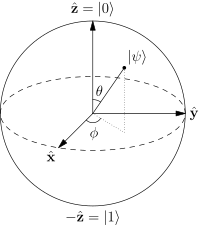
\includegraphics[width=0.3\columnwidth]{Bloch.png}
    \caption{Bloch sphere representation of a qubit}
    \label{fig:Bloch-Sphere}
\end{figure}

\subsubsection{Wigner Function}
The \textit{Wigner function} is the \textit{distribution} in the \textit{phase space} of a continuous variable quantum system\footnote{Such as position and momentum}. For classical systems, phase space distributions correspond to a classical probability distribution. However, the Wigner function the distribution also involves quantum uncertainty. Wigner functions can take on negative values in small regions, and are therefore quasi-probability distributions. This is allowed, since only areas larger than $\hbar$ are ever allowed to be measured, according to the Heisenberg uncertainty principle.

The Wigner function of a particle with wave function $\psi (q)$, is defined as 
\[
    W (q, p) := \frac{1}{\pi \hbar} \int_{-\infty}^\infty \psi^* (q + y) \psi (q - y) e^{\frac{2ipy}{\hbar}} dy
\]
An interesting example to use of the Wigner function is looking at the Wigner function of a Fock state. The Wigner distribution of a Fock state could be calculated directly from definition and the resulting expression is\footnote{proof of which is left as an exercise to the reader ;)}
\[
    W_n = \frac{2}{\pi} (-1)^n L_n[4 (q^2 + p^2)]e^{-2 (q^2 + p^2)}
\]
More importantly, we can look at a heat map of the Wigner function, as a nice visual aid to understand the state. An example of the $\ket{4}$ state Wigner distribution is shown in figure \ref{fig:Fock-State-Wigner}
\begin{figure}[H]
    \centering
    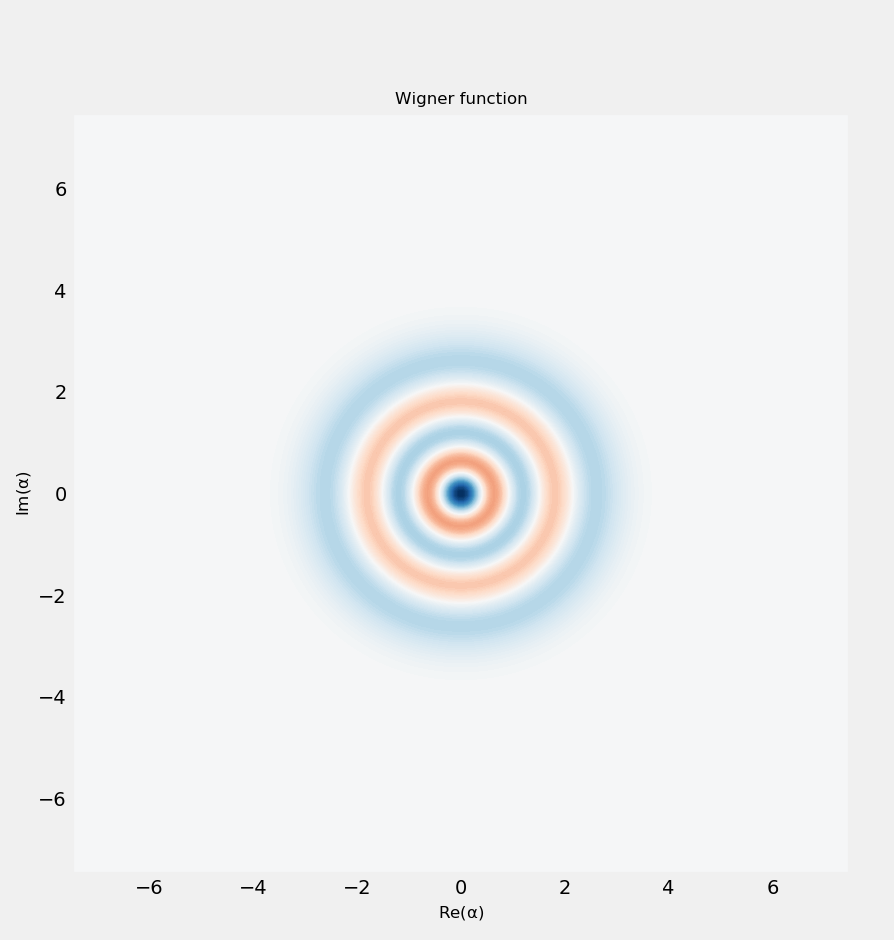
\includegraphics[width=0.3\columnwidth]{Wigner.png}
    \caption{Wigner distribution of the $\ket{4}$ Fock state}
    \label{fig:Fock-State-Wigner}
\end{figure}

\subsection{References and Further Readings}
The standard introductory book on this subject (which is also the one I used for reference) is "\textbf{Introductory Quantum Optics}" by Christopher C. Gerry and Peter L. Knight.

Another great resource is the series of online lectures taught by Prof. Alain Aspect from École Polytechnique.